\documentclass{article}
\usepackage[utf8]{inputenc}
\newcommand{\ii}{{\bf i}}
\newcommand{\jj}{{\bf j}}
\newcommand{\kk}{{\bf k}}
\newcommand{\id}{{\bf 1}}
\newcommand{\hur}{\frac{\id+\ii+\jj+\kk}{2}}%The "Hurwitz point"
\newcommand{\hurwitz}{\Z\left[\hur,\ii,\jj,\kk\right]}%The set of Hurwitz integers
\usepackage{wrapfig}
\usepackage{calligra}

\usepackage[utf8]{inputenc}
\usepackage[dvips]{graphicx}
\usepackage{a4wide}
\usepackage{amsmath}
\usepackage{mathtools}
\usepackage{euscript}
\usepackage{amssymb}
\usepackage{amsthm}
\usepackage{amsopn}
\usepackage[colorinlistoftodos]{todonotes}
\usepackage{graphicx}
\usepackage[T1]{fontenc}
\newcommand\mybar{\kern1pt\rule[-\dp\strutbox]{.8pt}{\baselineskip}\kern1pt}

\usepackage{ulem}
\usepackage{xcolor}
\newcommand{\cs}[1]{\color{blue}{#1}\normalcolor}

%Matrix commands
\newcommand{\ba}{\begin{array}}
\newcommand{\ea}{\end{array}}
\newcommand{\bmat}{\left[\begin{array}}
\newcommand{\emat}{\end{array}\right]}
\newcommand{\bdet}{\left|\begin{array}}
\newcommand{\edet}{\end{array}\right|}
\newcommand{\inv}[1]{#1^{-1}}

%Environment commands
\newcommand{\be}{\begin{enumerate}}
\newcommand{\ee}{\end{enumerate}}
\newcommand{\bi}{\begin{itemize}}
\newcommand{\ei}{\end{itemize}}
\newcommand{\bt}{\begin{thm}}
\newcommand{\et}{\end{thm}}
\newcommand{\bp}{\begin{proof}}
\newcommand{\ep}{\end{proof}}
\newcommand{\bprop}{\begin{prop}}
\newcommand{\eprop}{\end{prop}}
\newcommand{\bl}{\begin{lemma}}
\newcommand{\el}{\end{lemma}}
\newcommand{\bc}{\begin{cor}}
\newcommand{\ec}{\end{cor}}
\newcommand{\lcm}{\mbox{lcm}}
\newcommand{\defn}{\fbox{definition}}
\newcommand{\prop}{\fbox{proposition}}
\newcommand{\stab}{\mbox{stab}}
\newcommand{\Aut}{\mbox{Aut}}
\newcommand{\orb}{\mbox{orb}}

\newcommand{\norm}{\righttriangle}

\newcommand{\and}{\wedge}
\newcommand{\or}{\vee}



%sets of numbers
\newcommand{\N}{\mathbb{N}}
\newcommand{\Z}{\mathbb{Z}}
\newcommand{\Q}{\mathbb{Q}}
\newcommand{\R}{\mathbb{R}}

\newcommand{\topT}{\mathcal{T}}
\newcommand{\standtop}{\mathcal{T}_{STD}}
\newcommand{\cc}{\mathcal{C}}


\documentclass{article}
\usepackage[utf8]{inputenc}
\newcommand{\ii}{{\bf i}}
\newcommand{\jj}{{\bf j}}
\newcommand{\kk}{{\bf k}}
\newcommand{\id}{{\bf 1}}
\newcommand{\hur}{\frac{\id+\ii+\jj+\kk}{2}}%The "Hurwitz point"
\newcommand{\hurwitz}{\Z\left[\hur,\ii,\jj,\kk\right]}%The set of Hurwitz integers
\usepackage{wrapfig}
\usepackage{calligra}
\usepackage[utf8]{inputenc}
\usepackage[dvips]{graphicx}
\usepackage{a4wide}
\usepackage{amsmath}
\usepackage{euscript}
\usepackage{amssymb}
\usepackage{amsthm}
\usepackage{amsopn}
\usepackage[colorinlistoftodos]{todonotes}
\usepackage{graphicx}
\usepackage[T1]{fontenc}
\newcommand\mybar{\kern1pt\rule[-\dp\strutbox]{.8pt}{\baselineskip}\kern1pt}

\usepackage{ulem}
\usepackage{xcolor}
\newcommand{\cs}[1]{\color{blue}{#1}\normalcolor}

%Matrix commands
\newcommand{\ba}{\begin{array}}
\newcommand{\ea}{\end{array}}
\newcommand{\bmat}{\left[\begin{array}}
\newcommand{\emat}{\end{array}\right]}
\newcommand{\bdet}{\left|\begin{array}}
\newcommand{\edet}{\end{array}\right|}
\newcommand{\inv}[1]{#1^{-1}}

%Environment commands
\newcommand{\be}{\begin{enumerate}}
\newcommand{\ee}{\end{enumerate}}
\newcommand{\bi}{\begin{itemize}}
\newcommand{\ei}{\end{itemize}}
\newcommand{\bt}{\begin{thm}}
\newcommand{\et}{\end{thm}}
\newcommand{\bp}{\begin{proof}}
\newcommand{\ep}{\end{proof}}
\newcommand{\bprop}{\begin{prop}}
\newcommand{\eprop}{\end{prop}}
\newcommand{\bl}{\begin{lemma}}
\newcommand{\el}{\end{lemma}}
\newcommand{\bc}{\begin{cor}}
\newcommand{\ec}{\end{cor}}
\newcommand{\lcm}{\mbox{lcm}}
\newcommand{\defn}{\fbox{definition}}
\newcommand{\prop}{\fbox{proposition}}
\newcommand{\stab}{\mbox{stab}}
\newcommand{\Aut}{\mbox{Aut}}
\newcommand{\orb}{\mbox{orb}}

\newcommand{\norm}{\righttriangle}

\newcommand{\and}{\wedge}
\newcommand{\or}{\vee}



%sets of numbers
\newcommand{\N}{\mathbb{N}}
\newcommand{\Z}{\mathbb{Z}}
\newcommand{\Q}{\mathbb{Q}}
\newcommand{\R}{\mathbb{R}}

\newcommand{\topT}{\mathcal{T}}
\newcommand{\standtop}{\mathcal{T}_{STD}}
\newcommand{\cc}{\mathcal{C}}


\title{Topology}
\author{August bergquist}


\begin{document}

\maketitlea

\fbox{problem 1} Define the region $R$ as $R = [-2,2]\times [-1,1]\subseteq \R^2$, and define sub-regions $R_- = \{(x,y)\in R : -x + |y| \ge 1 \}$, $R_0 = \{(x,y\in R : |x| + |y| \le 1)\}$, and $R_+ = \{x + |y| \ge 1\}$.\\

\begin{itemize}
    \item[a. ] Find a bijective function $f:R\rightarrow R$ that maps points of $R_0$ onto $R_- \cup R_0$ and points of $R_0\cup R_+$ onto $R_+$. \\
    
    \fbox{solution} Consider the function  $f:R\rightarrow R$
    $$f(x,y) = 
    \begin{dcases}
    \Big( \Big[\frac{-|y|+3}{|y|+1}\Big](x+2)-2 ,y\Big) & (x,y)\in R_- \\
    \Big( \Big[\frac{|y| + 1}{-|y|+3}\Big](x-2)+2 ,y\Big) & (x,y)\in R_0 \cup R_+ 
    \end{dcases}.
    $$
    
    It remains to be shown that (1) $f$ is well defined, (2) $f$ actually maps $R_-$ onto $R_- \cup R_0$ and $R_0\cup R_+$ onto $R_+$, and (3) $f$ is bijective. Showing that $f$ is bijective will show the onto part of (2), hence it will suffice to show that $R_-$ maps to $R_-\cup R_0$ and $R_0\cup R_+$ maps to $R_+$.\\
    
    \begin{enumerate}
        \item First, notice that the cases by which $f$ is defined are not disjoint, their intersection being points in $R_- \cup R_0\cup R_+$. These will be points in $R$ such that $|y| = x + 1$. For ease of reference, call the case where $(x,y)\in R_-$ case A, and the other case B. Substituting $|y| = x + 1$ into the formula for case $A$, we obtain for the first coordinate
        $$\Big[\frac{-|y|+3}{|y|+1}\Big](x+2)-2 = \Big[\frac{-(x+1)+3}{(x+1)+1}\Big](x+2)-2 = -x.$$
        Furthermore, $y$ maps to $y$ in case $A$, so the image of $(x,y)\in R_-\cap (R_0\cup R_+)$ in case $A$ is $(-x,y)$.\\
        
        Likewise, for the first coordinate in case B, $x$ maps to 
        $$ \Big[\frac{(x+1) + 1}{-(x+1)+3}\Big](x+2)-2 = -x.$$
        Also, it is clear from the definition of $f$ that the second coordinate maps to $y$. So the image of $(x,y)\in R_-\cap (R_0\cup R_+)$ in case $B$ is $(-x,y)$. This is the same as in case $A$, so we conclude that on the intersection of cases $A$ and $B$, $f$ is still well defined. Hence $f$ is well defined. \\
        
        \item Now to show that $R_-$ maps to $R_-\cup R_0$, let $(x,y)$ be arbitrary in $R_-$. By definition of $R_-$, $-2 \le x \le |y| + 1$. Hence $0 \le x + 2 \le |y| + 1 $. Since $$\frac{-|y|+ 3}{|y| + 1} \ge 0 \mbox{   } \forall y \mbox{ s.t. } |y| \le 2$$ it follows that 
        $$(|y| + 1)\Big(\frac{-|y|+3}{|y| + 1}\Big) = -|y| + 3 \ge \Big(\frac{-|y| + 3}{|y|+1}\Big)(x + 2) \ge 0.$$
        Hence 
        $$1-|y| \ge \Big(\frac{-|y| + 3}{|y|  +1}\Big)(x+2) - 2 \le -2.$$
        Since obviously $-2\le y \le 2$, and since $f(x,y) = \Big(\frac{-|y| + 3}{|y|  +1}\Big)(x+2) - 2$, it follows that 
        $$f(x,y)\in R_-\cup R_0.$$
        
        We can use a similar, and similarly tedious argument to show that $R_0$ really does map to $R_0\cup R_-$. See the handwritten calculations.
        \item Finally, we must find an inverse. Consider the function $q:R\rightarrow R$ defined 
        $$q(x,y) = \begin{dcases}
        \Big(\Big[\frac{|y| + 1}{-|y| + 3}\Big](x-2) + 2,y\Big) & (x,y)\in R_-\cup R_0\\
        \Big(\Big[\frac{-|y|+3}{|y| + 1}\Big](x + 2) - 2,y\Big) & (x,y)\in R_+
        \end{dcases}$$
        for all $(x,y)\in R$.
        To show that $q$ really is the inverse of $f$, we must consider its left and right composition with $f$. In the hand-written notes I have evaluated each case.
    
    \end{enumerate}
    \item[b. ] Show that $f$ is a homeomorphism from $R$ onto itself.\\
    
    \fbox{proof} We have already shown that $f$ has an inverse and is bijective. It remains to be shown that $f$ is continuous, and that $f$'s inverse is as well. We are assuming that functions in subsets of $\R^2$ are continuous if their individual coordinates are continuous. In the interior of $R_-$ $R_0\cup R_+$, continuity of the first coordinate is ensured by the fact that rational functions are continuous, so long as the denominator is nonzero. Since the only denominators are $|y| + 1$ and $-|y| + 3$, the first of which is never zero, and the second which is zero only when $y=\pm 3$, which can never happen in $R$, it follows that the first component of $f$ is continuous on the interiors of $R_-$ and $R_0\cup R_+$. Furthermore, $y \rightarrow y$ is continuous, since it is linear. We need only be concerned about the boundary of $R_-$ and $R_0\cup R_+$. Since $f$ is continuous throughout $R_-$, the limit from the left as $(x,y)$ approaches the intersection of $R_-$ and $R_0\cup R_+$ must be $f(x,y)$. Likewise from the right. Since we have already shown that $f(x,y)$ is well defined on this boundary, it follows that $f$ is continuous there also.
    
    Hence $f$ must be continuous. Furthermore, since $f^{-1} = q$ is also a rational function with the same denominators, and in the same region, hence these denominators can never be zero. So $q$ is continuous as well.
    
    \item Show that $g:\R^2\rightarrow \R^2$ defined
    $$g(x,y) = \begin{dcases}
    f(x,y) & (x,y)\in R\\
    (x,y) & (x,y)\in \R^2-R
    \end{dcases}$$ is a homeomorphism from $\R^2\rightarrow \R^2$.\\
    
    \fbox{solution} We can tell right off the bat that $g$ is well defined, as the identity map and $f$ are well defined, and $R\cap (\R^2-R)$ is disjoint. To show that $g$ is bijective, consider the function $$
    h(x,y) = 
    \begin{dcases}
    q(x,y) & (x,y)\in R\\
    (x,y) & (x,y)\in \R^2 - R.
    \end{dcases}.$$
    Evaluating $h\circ g(x,y) = h(g(x,y))$, we have two cases. The first is trivial: if $(x,y)\in \R^2- R$, then $h\circ g(x,y) = h(g(x,y)) = h(x,y) = (x,y)$. Suppose then that $(x,y)\in R$. Then the proof that $h(x,y)$ in this case really is an inverse reduces to the proof that $q(x,y)$ is really its own inverse.\\
    
    The fact that $g$ and $h$ really are continuous follows from the fact that on the boarder of the region $R$, $f$ and $\inv{f}$ act as the identity. The scaling factors $r = \frac{|y|+ 1}{-|y| + 3}$ and $1/r$ become $1$ when $|y| = 1$. The thing being scaled by becomes $0$ (since $(x+2)$ is zero in $R_-$ when $x = -2$, and likewise for $(x-2)$ in $R_+$), leaving us with $0-2 = -2 = x$ and $ 0 + 2 = 2 = x $ for both piecewise cases of $f$ in $R_-$ and $R_+$ respectively. Also, $y$ gets mapped to $y$ regardless.
    
    Since $g$ is a continuous bijection from $\R^2$ to $\R^2$, whose inverse is also continuous, it follows that $g$ is a homeomorphism.
\end{itemize}

\newpage

\begin{figure}[htbp]
\centerline{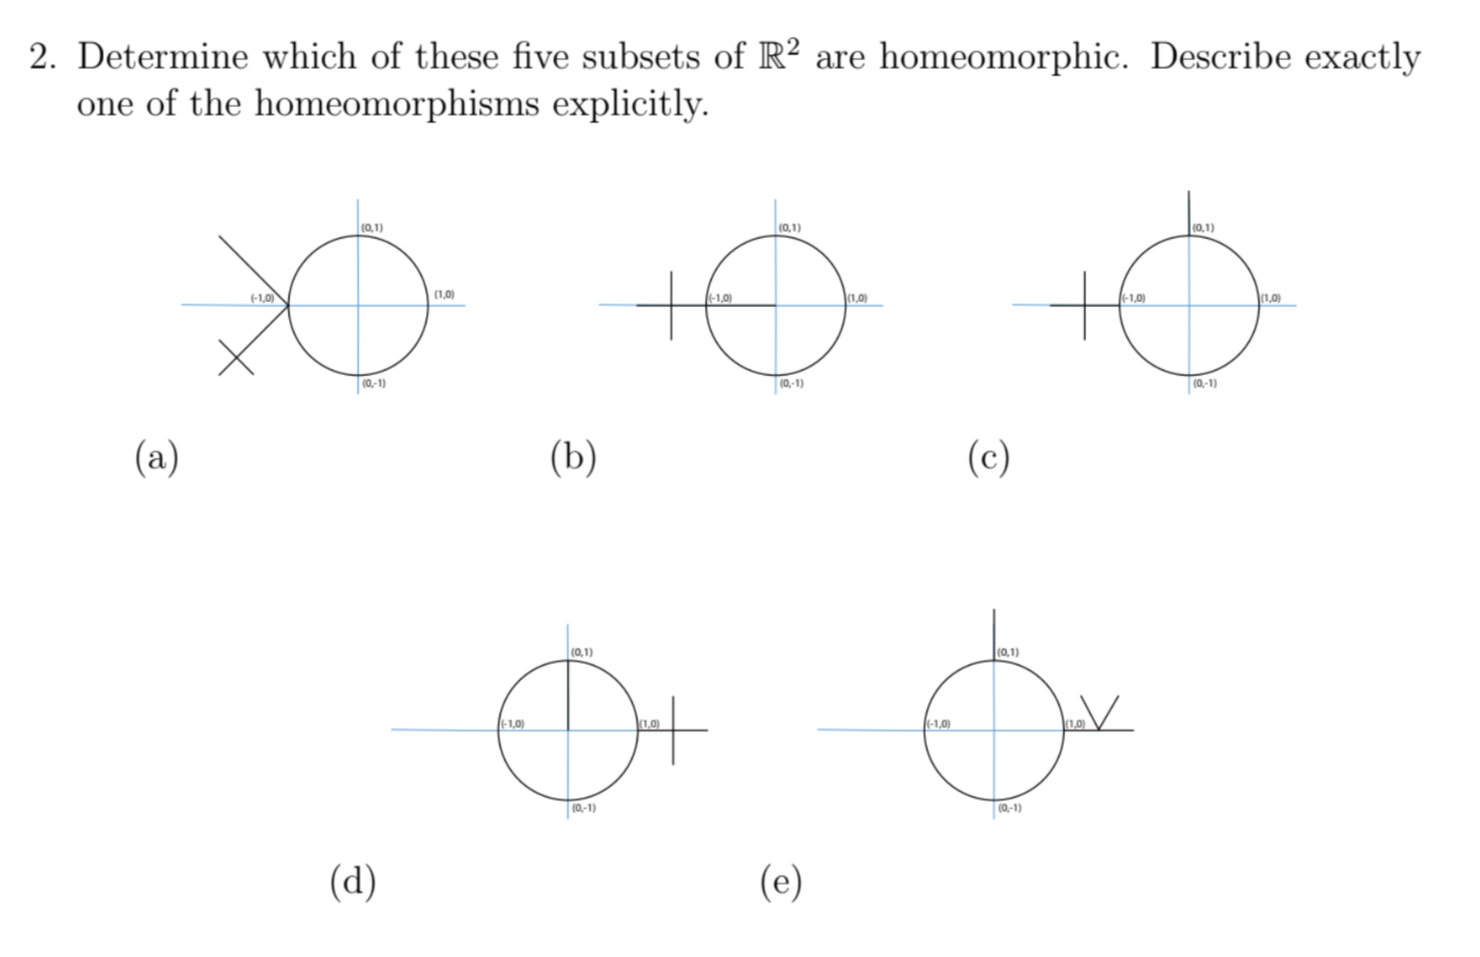
\includegraphics[scale=0.5]{homework/circles.png}}
\caption{}
\label{fig}
\end{figure}

\fbox{problem 2} Decide which of the above are homeomorphic. Find an explicit homeomorphism between two of them.\\

\fbox{solution} Intuitively, we can see that $a$ and $b$ must be homeomorphic, as we can imagine rotating the cross arm clockwise 45 degrees onto the $x$-axis, and the straight arm 135 degrees counterclockwise, also onto the $x$ axis. Notice that this process didn't involve any cutting or tearing, and intuitively it is continuous. \\

Furthermore, $c$, $d$, and $e$ must also be homeomorphic. By the transitivity and symmetry of homeomorphisms, intuitively showing that $c$ is homeomorphic to $d$, and $c$ to $e$, we would get the whole job done all at once. We will ignore the homeomorphism from $c$ to $d$, as we will soon describe it explicitly. Rotate the leftmost part of the $v$ shape about 20 degrees clockwise, so that it is perpendicular to the $x$-axis. Rotate the other arm by about 130 degrees counterclockwise until it too is perpendicular to the $x$-axis. Reflect $c$ across the $y$ axis. Notice now that $e$ has been transformed into $c$, and that in this process no cutting or tearing was involved. It is also bijective because we could reverse all of the steps we have taken.
\\

Now we will describe the homeomorphism from $c$ to $d$ explicitly. A few guiding notes will be helpful before we begin. First, let the line that sticks up from the circle be denoted as $L$. Let the rest be denoted as $C$, and the whole thing be denoted as $R$. We will refer to the whole thing in $d$ as $R'$. Hence we will need to find a homeomorphism $f:R\rightarrow R'$. Furthermore, denote the "hanging" line in $d$ as $L'$, and the rest of $R'$ including the top of the circle as $C'$.\\

Consider the function $f:R\rightarrow R'$, defined 
$$
f(x,y) = \begin{dcases}
(x,2-y & (x,y)\in L\\
(-x,y) & (x,y)\in C
\end{dcases}
.$$

From the picture, we can see that the intersection of $L$ and $C$ is non-empty, for they intersect at the point $(0,1)$. To show that $f$ is well defined, we will need to show that in both cases, $f$ maps to the same thing. In the first case, $f(0,1) = (0,2-1) = (0,1)$. In the second case, $f(0,1) = (0,1)$, which is consistent with the first value for $f(0,1)$. Since $(0,1)$ is the only point where the two regions of definition for $f$ intersect, and since both definitions agree there, it follows that $f$ is well defined. \\

In order to show that $f$'s codomain is really as claimed, and that $f$ is bijective, we will need a more explicit description of $L$, $C$, $L'$, and $C'$. Let $C = \{(x,y)\in \R^2:x^2 + y^2 = 1\}\cup \{(x,y)\in \R^2: y = 0, -1\le x\le 0 \}\cup \{(x,y)\in \R^2: x = -3/2, -1/2 \le y \le 1/2 \}$. Let $L = \{ (x,y)\in \R^2 : x = 0, 2\le y \le 3 \}$. We define $R = L\cup C$.\\

We also define $C' = \{(x,y)\in \R^2 : x^2 + y^2 = 1\}\cup \{(x,y)\in \R^2 : y = 0, 0\le x \le 1\}\cup \{(x,y)\in \R^2 : x = 3/2, -1/2 \le y \le 1/2\}$ and $L' = \{(x,y)\in \R^2: 0\le x\le 1\}$.\\

To show that $f$ really maps to $R'$. There are two cases: either $(x,y)\in L$ or $ (x,y)\in C $.
\begin{enumerate}
    \item Suppose that $(x,y)\in L$. Well then, by definition of $L$, $x = 0$ and $2\le y \le 3$. Then multiplying all sides by $-1$ we have $-3 \le -y \le -2$. Adding one on all sides, we have $2-3 \le 2-y \le -2$. By definition of $f(x,y)$, and since $(x,y)\in L$, and by definition of $L'$ it follows that $f(x,y)\in L'$. This is good.\\
    \item Now suppose that $(x,y)\in C$. Manipulating the inequalities, we find that $f(x,y)\in C'$.
\end{enumerate}

To show that $f$ really is bijective, we notice that $f$ is almost its own inverse. Consider the function
$$\inv{f} = \begin{dcases}
(x,2-y) & (x,y)\in L'\\
(-x,y) & (x,y)\in C'
\end{dcases}$$

The fact that this really is the inverse is apparent from the fact that $f$ maps $L\rightarrow L'$ and $C\rightarrow C'$, and that both of these mappings are reflections. The repeating of a reflection is always the identity map.\\

The continuity of $f$ and $\inv{f}$ is assured by the fact that the function is composed of linear functions in both piecewise cases, which are also continuous, and that the $f$ agrees on the intersection of these both cases. Remember that if a function is continuous, it's limit at a given value must be the actual value of the function.

\end{document}